\documentclass[tikz,border=10pt]{standalone}
\usepackage{tikz}
\usetikzlibrary{calc,patterns,decorations,decorations.pathreplacing,shapes.arrows}

\begin{document}

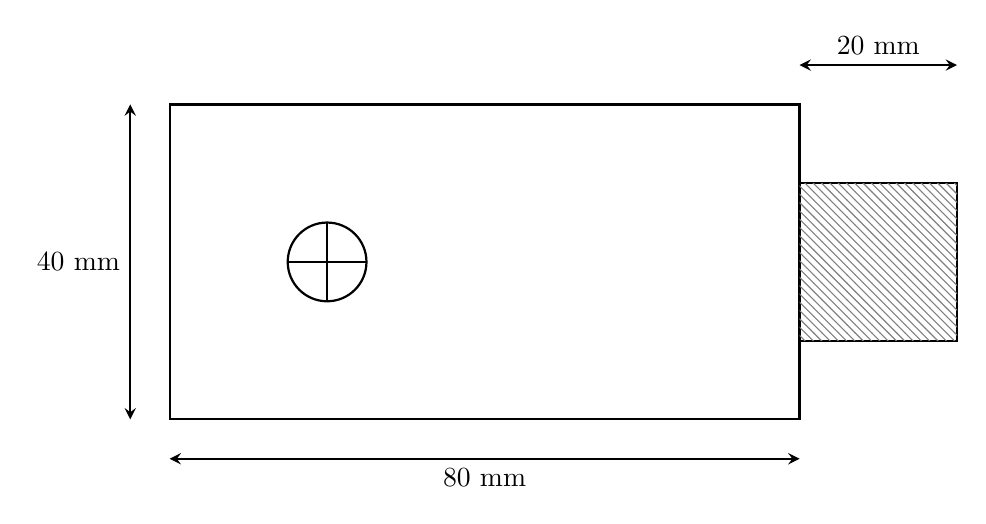
\begin{tikzpicture}

    % Define some common styles
    \tikzset{
        dimline/.style={thick, >=stealth},
        hidden/.style={dashed},
        section/.style={pattern=north west lines, pattern color=black!50}
    }
    
    % Draw the base rectangle (main body)
    \draw[thick] (0,0) rectangle (8,4);
    
    % Draw a circular hole
    \draw[thick] (2,2) circle (0.5);
    
    % Draw a side extension
    \draw[thick] (8,1) -- (10,1) -- (10,3) -- (8,3);
    
    % Add hidden lines (dashed)
    \draw[hidden] (2,1.5) -- (2,2.5);
    
    % Dimension lines
    \draw[dimline,<->] (0,-0.5) -- (8,-0.5) node[midway, below] {80 mm};
    \draw[dimline,<->] (-0.5,0) -- (-0.5,4) node[midway, left] {40 mm};
    \draw[dimline,<->] (8,4.5) -- (10,4.5) node[midway, above] {20 mm};
    
    % Center mark for the hole
    \draw[dimline] (2,1.5) -- (2,2.5);
    \draw[dimline] (1.5,2) -- (2.5,2);
    
    % Section pattern
    \fill[section] (8,1) rectangle (10,3);

\end{tikzpicture}

\end{document}
